\apendice{Documentación de usuario}

\section{Introducción}

\section{Requisitos de usuarios}

\section{Instalación}


	\begin{figure}%[!h]
		\centering
		\includegraphics[width=0.9\textwidth]{#1}
		\caption{#2}\label{fig:#1}
	\end{figure}

\section{Manual del usuario}

Intro.......




En primer lugar es necesario crear la Base de Datos denominada BBDD donde se almacena la estructura de tablas del proyecto.
Para crearla únicamente es necesario pulsar sobre el Botón {Crear BBDD} situado en el menú superior de la aplicación, en \emph{Configuración}(figura \ref{fig:crearBBDD}).

\begin{figure}%[!h]
		\centering
		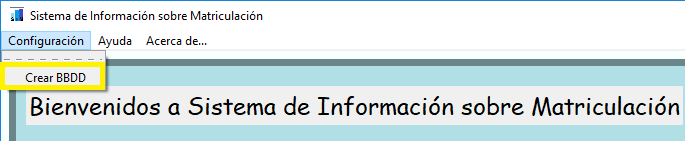
\includegraphics[width=0.9\textwidth]{crearBBDD}
		\caption{Botón de creación de la Base de Datos}\label{fig:crearBBDD}
	\end{figure}


Al pulsar sobre este botón se creará la Base de Datos y por consiguiente el fichero BBDD en la ruta donde estemos ejecutando la aplicación.
Si es la primera vez que pulsamos este botón, se creará con éxito; pero si ya existiera la BBDD, se nos mostraría un mensaje de \emph{Warning} como el de la figura \ref{fig:warningBBDD}. 
\begin{figure}%[!h]
		\centering
		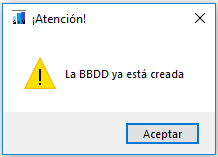
\includegraphics[width=0.5\textwidth]{warningBBDD}
		\caption{Mensaje de \emph{Warning} de BBDD ya creada}\label{fig:warningBBDD}
	\end{figure}


De esta forma, no se volverá a crear la Base de Datos y mantendremos nuestra BBDD anterior.

Una vez creada la BBDD, necesitamos rellenarla de datos. Para esta labor, se utilizan ficheros de datos de matriculación de alumnos descargados de \emph{Sigma}.

Ya se han explicado los problemas que existen con estos tipos de ficheros en [xxxxxxxxxxxxxxxxxxxxxxxxx].
Por esta razón, estos ficheros se deben parsear y preprocesar antes de añadir a la BBDD. Para esta labor, contamos con el botón de \emph{Preprocesar}. Este botón se ubica en la pantalla principal de la aplicación, ya que es un botón que se utilizará con cierta normalidad y periodicidad. 

\begin{figure}%[!h]
		\centering
		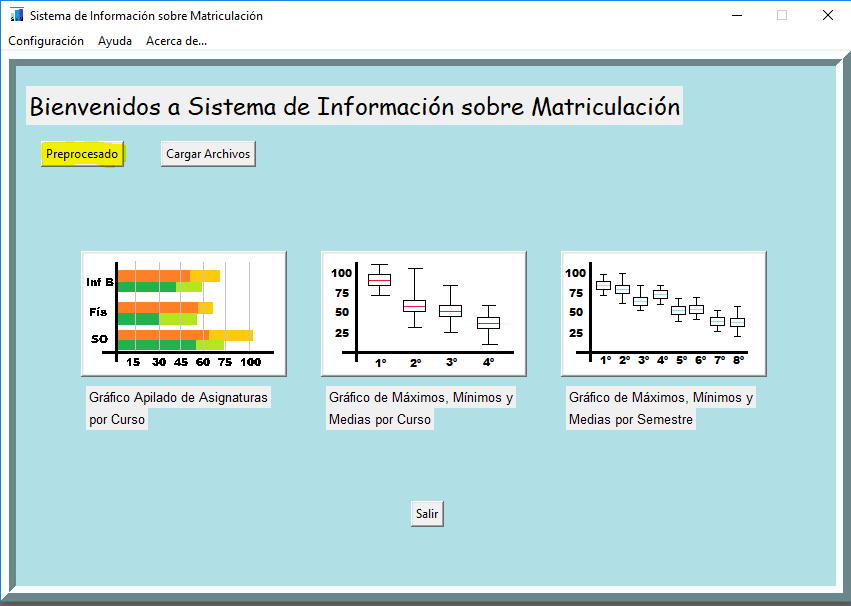
\includegraphics[width=\textwidth]{preprocesar}
		\caption{Mensaje de \emph{Warning} de BBDD ya creada}\label{fig:preprocesar}
	\end{figure}



Cuando pulsamos este botón (\ref{fig:preprocesar}), se mostrará una ventana del Sistema Operativo, donde se nos permitirá seleccionar archivos (.xls) únicamente.


\begin{figure}%[!h]
		\centering
		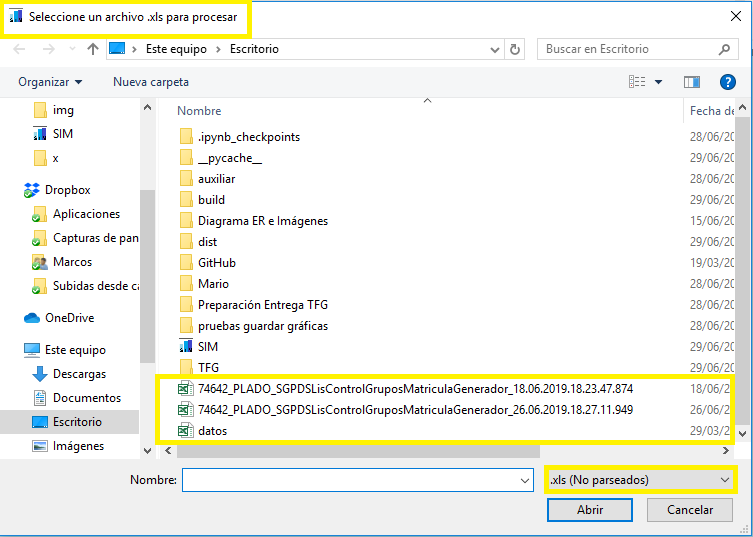
\includegraphics[width=\textwidth]{ventanaSOxls}
		\caption{Ventana del Sistema Operativo}\label{fig:ventanaSOxls}
	\end{figure}


Seleccionamos el archivo que deseemos (deben ser archivos descargados de {Sigma}) y pulsamos abrir.
Una vez realizado esto, se generará en la misma ruta un fichero con extensión (.csv) corregido, modificado y preparado para la carga de datos en la BBDD.

(imagen del fichero csv generado)

En este punto, ya podemos realizar la carga de datos. Para eso contamos con un botón de {Cargar Archivos} situado en la pantalla principal de la aplicación.

(boton cargar archivos)

De la misma forma que el anterior paso, cuando pulsamos este botón, se mostrará una ventana del Sistema Operativo, donde se nos permitirá seleccionar 
archivos (.csv) únicamente.

(ventanaSOxls)

Seleccionamos el archivo que se ha generado en el paso anterior y pulsamos abrir.
Una vez realizado esto, se procederá a realizar la carga de todos los datos del fichero a la BBDD.

En este punto, ya contamos con información o datos para realizar los diferentes tipos de gráficas.

Por lo tanto pulsamos en uno de los 3 tipos de gráficos (el primero por ejemplo) y se nos abrirá una nueva ventana.


En esta ventana, se muestran una serie de desplegables con la información necesaria para que el usuario seleccione para la realización de ese
 tipo de gráfico específico. Hay que destacar que en cada desplegable se muestra toda la información diferente que se encuentre en la BBDD.
(foto pantalla Grafico 1 con desplegable abierto)

Para obtener correctamente el gráfico, es necesario seleccionar una opción de cada desplegable.
Una vez seleccionado el Año, Titulación y Curso































